% =========================================================
% Section 7 (Final Trim): Sensitivity & Robustness (O-Award audit style)
% Target length: ~1.0–1.5 pages (single-column MCM template)
% =========================================================

\section{Sensitivity Analysis and Model Robustness Checks}
\label{sec:robustness}

\textbf{Audit objective.}
All Q2--Q4 claims are \emph{posterior-averaged} functionals propagated from Q1 (Monte Carlo, $M=2000$). We therefore audit robustness along three axes: \textbf{(i) statistical stability + Bayesian prior defense} (Q1--Q2), \textbf{(ii) structural invariance to model class} (Q3), and \textbf{(iii) mechanism resilience with a stability region (not ``magic numbers'')} (Q4), plus explicit safe-operation constraints.

\vspace{-0.35em}
\subsection{Statistical stability \& prior defense (Q1--Q2)}
\vspace{-0.35em}

Define the prefix-to-full convergence diagnostic
\begin{equation}
\Delta_{L1}(M')=\left\|\bar v_{M'}-\bar v_{2000}\right\|_1,
\label{eq:l1def}
\end{equation}
where $\bar v_{M'}$ is the posterior mean fan-share vector computed from the first $M'$ draws. On the audited corner week (S27W8), $\Delta_{L1}(800)=2.225\times10^{-3}$ and $\Delta_{L1}(1500)=1.323\times10^{-3}$ (Fig.~\ref{fig:robust_panels}a), indicating that $M=2000$ lies in the plateau regime and downstream summaries are not driven by finite-sample Monte Carlo error.
The posterior is constraint-dominated:
\[
p(v_{s,t}\mid\cdot)\ \propto\ \pi_{\beta}(v_{s,t})\cdot \mathbf{1}\{v_{s,t}\in\mathcal{A}_{s,t}\},
\]
so feasibility $\mathcal{A}_{s,t}$ shapes posterior mass more strongly than the Dirichlet curvature. On S27W8, a prior sweep over $\beta\in\{0,0.5,1,2,5\}$ (Base=$\beta=0$ uniform) yields stable summaries: the posterior mean shifts only $0.2027\to0.1997$ ($\approx$1.5\%), the CI width remains within 0.0670--0.0685, and the anomaly rank remains 1 (Table~\ref{tab:prior_sens_short}), addressing the prior-sensitivity concern.

Rule comparisons are computed over the full posterior ensemble. Rank vs.\ Percent differs non-trivially ($P_{\mathrm{diff}}=0.260$, $D_{\exp}=0.485$), and in the Agency regime Percent improves alignment and global consistency ($FAI_{\mathrm{Pct}}=0.277$, $\rho_{\mathrm{Pct}}=0.765$); thus the conclusion is supported at the distribution level rather than by posterior means alone.


\vspace{1ex}


\vspace{-0.45em}
\begin{table}[H]
\centering
\caption{Prior sensitivity audit (Q1, S27W8; Base=$\beta=0$ uniform). The anomaly signal is stable across a wide prior grid, indicating constraint-dominated inference.}
\label{tab:prior_sens_short}
\scriptsize
\setlength{\tabcolsep}{15.3pt}  
\renewcommand{\arraystretch}{0.93}
\begin{tabular}{@{}cccccc@{}}
\toprule
$\beta$ & Accept & Mean & 95\% CI & Rank & $L_1$ vs.\ Base \\
\midrule
0.0 & 0.2098 & 0.2027 & [0.1744,0.2414] & 1 & 0.0000 \\
0.5 & 0.2227 & 0.2026 & [0.1741,0.2414] & 1 & 0.0027 \\
1.0 & 0.2345 & 0.2023 & [0.1739,0.2411] & 1 & 0.0062 \\
2.0 & 0.2610 & 0.2015 & [0.1731,0.2415] & 1 & 0.0130 \\
5.0 & 0.3266 & 0.1997 & [0.1703,0.2388] & 1 & 0.0350 \\
\bottomrule
\end{tabular}
\vspace{-1.0em}
\end{table}

\vspace{-0.25em}
\subsection{Methodological invariance (Q3)}
\vspace{-0.35em}

\noindent ``Dual-Protection'' survives a change of hypothesis class: a parametric discrete-time hazard model and a non-parametric Random Forest both prioritize \emph{fan support} ($YV$) and \emph{technical score} ($YJ$) as dominant protective drivers. Quantitatively, among shared substantive covariates $\{YV,YJ,\mathrm{age}_c,\mathrm{age}_c^2,\mathrm{tenure},\mu_J\}$, the rank agreement between hazard effect magnitudes and RF importances is $\rho_S=0.657$ (Spearman), supporting \textbf{driver hierarchy invariance} rather than functional-form dependence.

\vspace{-0.15em}
\subsection{Mechanism resilience \& stability region (Q4)}
\vspace{-0.35em}

Bobby Bones serves as an extreme-value validation: under the Percent baseline the case is effectively popularity-protected, whereas PAGS activates the safeguard and yields $p_{\mathrm{elim}}^{\mathrm{PAGS}}=0.856$, indicating correction under reputational-risk extremes.

Across perturbations, $\gamma$ primarily governs activation frequency without inducing systematic distortion: $\rho_S(\gamma,D)=-0.056$ ($p=0.362$), while $\rho_S(\gamma,\mathbf{1}_{\text{guardrail}})=0.186$ ($p=0.0024$). Activation is $0$ for $\gamma\le0.95$ (n=24) and $0.292$ for $\gamma>0.95$ (n=240), suggesting an empirical transition; Fig.~\ref{fig:robust_panels}b delineates a contiguous region over $(\gamma,w)$ in which activation is tunable and distortion remains bounded, mitigating concerns of ad hoc threshold dependence.

The safe-operation logic is summarized by three flagged conditions. Low-variance judge weeks warrant disabling z-score triggering and reverting to standard Percent to avoid hypersensitive activation. Save-era weeks motivate restricting PAGS to within-tier correction rather than claiming full-field reordering. Weak identifiability (unusually low acceptance or wide posteriors) warrants an audit-only flag and avoidance of high-stakes intervention.

Collectively, these audits support that Percent (agency), Dual-Protection (driver hierarchy), and PAGS (tail-risk safeguard) remain robust and interpretable under the stated constraints.


% -------------------------
% Two compact figure placeholders side-by-side (space-efficient)
% -------------------------
\vspace{-0.55em}
\begin{figure}[H]
\centering
\begin{minipage}{0.5\linewidth}
  \centering
  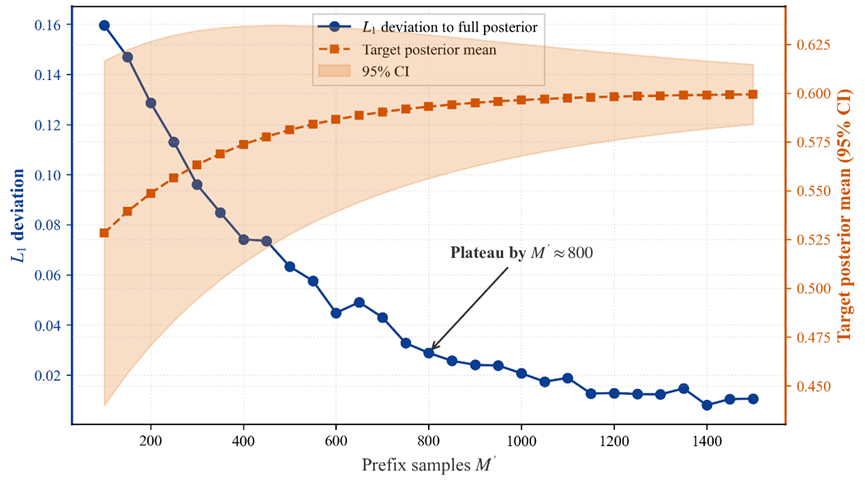
\includegraphics[width=0.95\linewidth]{figures/S1.png}
\end{minipage}\hfill
\begin{minipage}{0.5\linewidth}
  \centering
  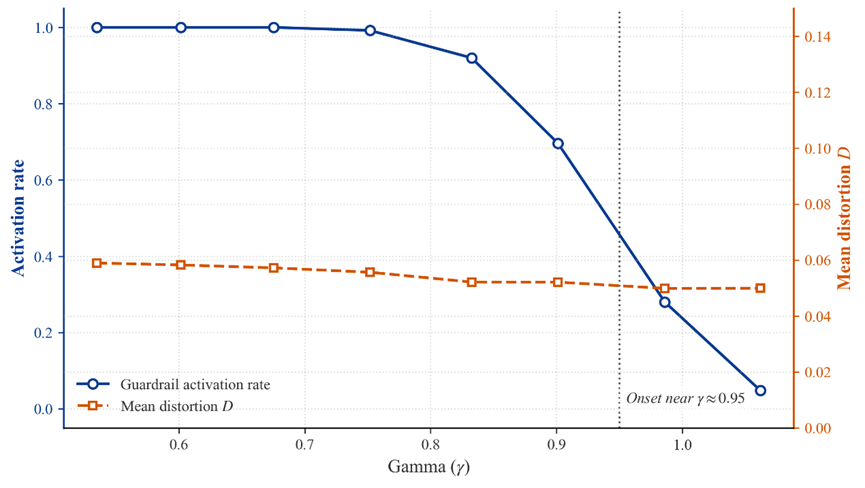
\includegraphics[width=0.95\linewidth]{figures/S2.png}
\end{minipage}
\caption{Compact robustness visuals for rapid audit.}
\label{fig:robust_panels}
\vspace{-1.0em}
\end{figure}

